\section{Supplementary material}

All reported appendix scores use IMD as the observational reference and the
same dates, grid, anomaly normal, and fractional-area support as the main
paper. No IMERG or temperature result is included in the current claims.

\subsection{Forecast inventory and coverage}

\begin{table*}[h]
\centering\small
\caption{Forecast cohort. The 2024 common intersection contains 30 cases;
2020--2023 and 2025 contain 35 per year. Operational ensemble size changes
where shown do not alter the ensemble-mean evaluation contract.}
\label{tab:inventory}
\resizebox{0.78\textwidth}{!}{\begin{tabular}{llrrr}
\toprule
System & Type & Members & 2020--23 cases/year & 2025 cases \\
\midrule
CMA operational & physics & 4 & 35 & 35 \\
DLESyM v0 & AI Earth system & 1 & 35 & 35 \\
ECMWF operational & physics & 51 or 101 & 35 & 35 \\
FuXi-S2S & AI subseasonal & 50 & 35 & 35 \\
NCEP operational & physics & 16 & 35 & 35 \\
NeuralGCM & hybrid AI--physics & 10 & 35 & 35 \\
UKMO operational & physics & 4 & 35 & 35 \\
\bottomrule
\end{tabular}
}
\end{table*}

The five missing 2024 common initializations are June 6, 10, 13, 17, and
August 5. Exact ISO dates are stored in \texttt{coverage.csv}; per-system
availability, coordinates, units, and source metadata hashes are stored in
\texttt{preflight/coverage\_preflight.csv} and
\texttt{preflight/preflight.json}. The metadata-only coverage preflight
records \texttt{forecast\_values\_read=false}. DLESyM and NeuralGCM 2025 files
enter through native-file adapters after the same coordinate, unit, and
42-period completeness checks as the standardized stores.

\subsection{All systems and all lead weeks}

\begin{table*}[h]
\centering\scriptsize
\caption{Complete 2025 national score table. RMSE, MAE, and bias are in mm
day$^{-1}$; wet-area error is forecast minus observed weighted fraction at
1 mm day$^{-1}$. Negative support is the area-weighted fraction of evaluated
support below zero under the no-clipping policy.}
\label{tab:all-methods}
\resizebox{\textwidth}{!}{\begin{tabular}{lrrrrrr}
\toprule
Method & ACC $\uparrow$ & RMSE $\downarrow$ & MAE $\downarrow$ & Bias & Wet-area error & Negative support (\%) \\
\midrule
PiggyCast, full & 0.347 & 4.989 & 3.603 & -0.303 & 0.113 & 0.52 \\
PiggyCast, forecast only & 0.339 & 5.028 & 3.626 & -0.288 & 0.117 & 0.16 \\
Validation-weighted mean & 0.313 & 5.150 & 3.700 & -0.397 & 0.114 & 0.00 \\
Equal-weight mean & 0.307 & 5.174 & 3.715 & -0.428 & 0.114 & 0.00 \\
ECMWF & 0.305 & 5.240 & 3.822 & 0.253 & 0.107 & 0.00 \\
Per-lead 2024-RMSE-selected & 0.296 & 5.283 & 3.845 & 0.157 & 0.097 & 0.00 \\
FuXi-S2S & 0.276 & 5.683 & 4.014 & -0.363 & 0.047 & 0.00 \\
NeuralGCM & 0.236 & 5.694 & 4.094 & -0.429 & 0.099 & 0.00 \\
UKMO & 0.226 & 6.370 & 4.522 & 0.328 & 0.044 & 0.00 \\
CMA & 0.197 & 6.852 & 4.839 & -0.364 & 0.052 & 0.06 \\
NCEP & 0.154 & 6.421 & 4.538 & -1.471 & -0.013 & 0.02 \\
DLESyM v0 & 0.102 & 6.735 & 4.815 & -0.950 & 0.010 & 0.00 \\
Location/calendar only & 0.101 & 5.587 & 4.091 & -0.402 & 0.144 & 0.06 \\
\bottomrule
\end{tabular}
}
\end{table*}

\begin{figure*}[h]
  \centering
  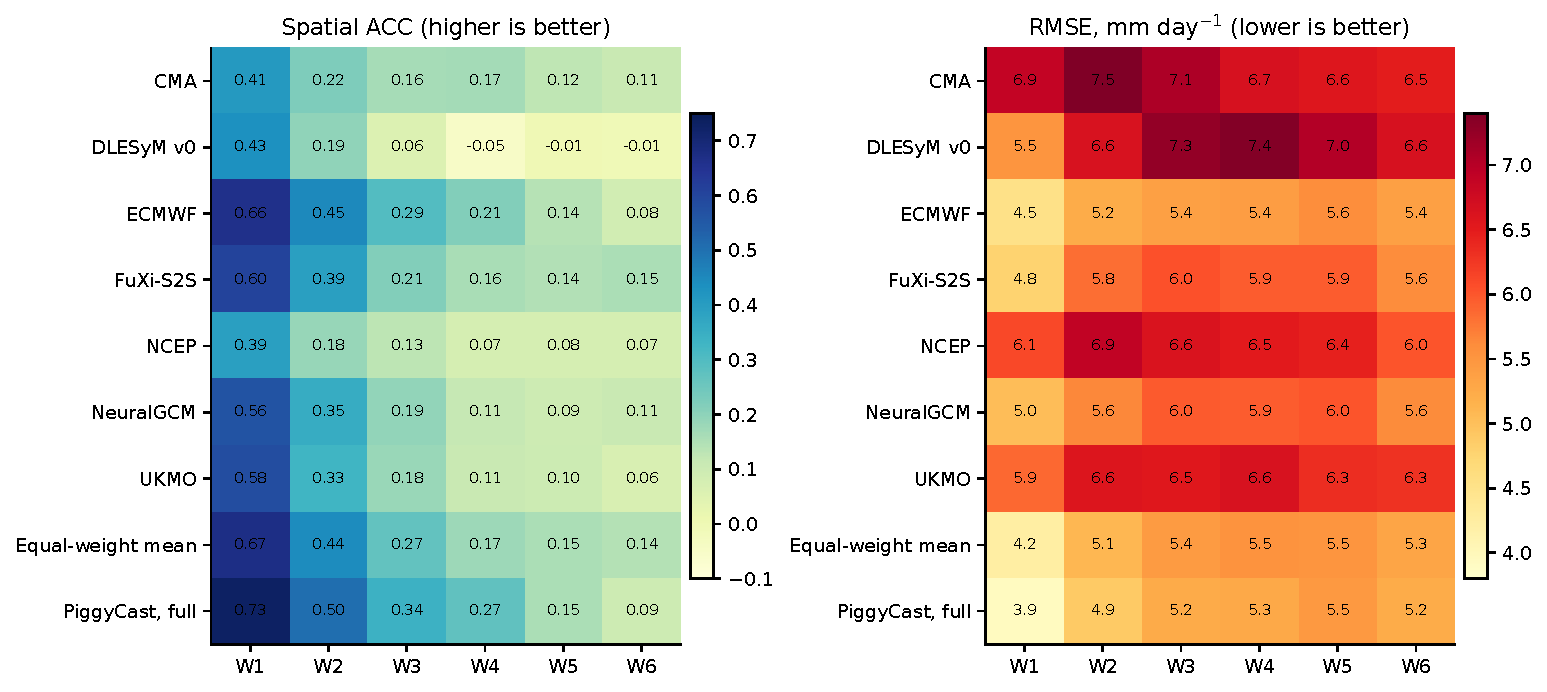
\includegraphics[width=\textwidth]{figures/appendix_all_models_imd.pdf}
  \caption{IMD-referenced 2025 national comparison for every base system,
  equal weighting, and full PiggyCast at Weeks 1--6. The defensible pattern is
  rapid, heterogeneous skill decay rather than a blanket statement that the
  systems are unskillful: several Week-1 forecasts have useful anomaly-pattern
  agreement, while Weeks 5--6 are consistently difficult.}
  \label{fig:all-models}
\end{figure*}

Figure~\ref{fig:all-models} replaces a visually crowded multi-line plot. It
also keeps ACC and RMSE together: a method can reduce rainfall-amplitude error
without improving the spatial anomaly pattern, as full PiggyCast does at the
longest leads.

\subsection{Regional and lead-wise behavior}

\begin{table}[h]
\centering\small
\caption{Full PiggyCast minus equal-weight regional ACC, averaged across
initializations and leads.}
\label{tab:regions}
\resizebox{\columnwidth}{!}{\begin{tabular}{lrrr}
\toprule
Domain: full $-$ equal weight & Mean & 2.5th pct. & 97.5th pct. \\
\midrule
india & 0.040 & 0.011 & 0.068 \\
northwest india & 0.128 & 0.085 & 0.177 \\
central india & 0.011 & -0.036 & 0.058 \\
south peninsula & 0.060 & 0.018 & 0.103 \\
east northeast india & -0.097 & -0.175 & -0.037 \\
\bottomrule
\end{tabular}
}
\end{table}

The lead-by-region diagnostic is shown in Figure~\ref{fig:effects} of the main
paper so that local lead-time failures are not hidden in the supplement.

\subsection{Claim gates and uncertainty}

The pre-specified headline requires positive lower 95\% ACC endpoints against
both equal weighting and the per-lead 2024-RMSE-selected baseline, a positive
forecast-only versus location/calendar-only endpoint, at most 5\% relative
RMSE regression, at most 0.5 mm day$^{-1}$ absolute-bias regression, and
positive regional ACC point differences in at least three of four regions.
All checks pass except the selected-baseline ACC endpoint. The regional point
gate should not be read as evidence of uniform benefit: only northwest and
south intervals exclude zero positively, while east/northeast excludes zero
negatively. The machine-readable decision is in
\texttt{gate\_report.json}.

\begin{table}[h]
\centering\small
\caption{95\% paired ACC intervals under alternative moving-block lengths.
Point effects are 0.040 (full minus equal) and 0.052 (full minus per-lead
selected) at every length.}
\label{tab:bootstrap}
\resizebox{\columnwidth}{!}{\begin{tabular}{rrr}
\toprule
Block length & Full $-$ equal & Full $-$ per-lead selected \\
\midrule
2 & [0.012, 0.067] & [0.009, 0.089] \\
4 & [0.011, 0.070] & [-0.002, 0.093] \\
8 & [0.017, 0.070] & [-0.002, 0.096] \\
\bottomrule
\end{tabular}
}
\end{table}

The equal-weight result is stable to the tested block lengths. The stronger
selected-baseline comparison is sensitive at its lower endpoint, which
motivates the conservative main-text interpretation.

\subsection{Preprocessing and quality control}

Daily precipitation is expressed as mm day$^{-1}$ before weekly averaging.
Each week requires seven finite daily periods; partial weeks are rejected.
Latitude order, longitude convention, initialization timestamps, accumulation
period endpoints, and ensemble dimensions are checked before scoring. The
same IMD observation fraction and fractional polygon overlap enter every
method's area weights. ACC is undefined for a case with zero weighted spatial
variance; such a case is recorded as missing rather than replaced by zero.

Small finite negative increments created when accumulated precipitation is
differenced are retained. Full PiggyCast has
\FullNegativePercent{}\% negative area-weighted national support overall. This
choice avoids a test-informed clipping rule and exposes a calibration issue
for future work.

\subsection{Hyperparameters and compute}

XGBoost uses squared-error loss, histogram trees on CPU, maximum depth 4,
minimum child weight 5, learning rate 0.03, row subsampling 0.8, column
subsampling 0.9, $L_2$ regularization 1, seed 42, and at most 600 trees with
patience 50. Exact selected tree counts, feature names, weighted row counts,
and serialized model paths for all 18 lead--variant combinations are stored in
\texttt{fit\_metadata.json}. Runtime and energy were not instrumented
reliably, so no numerical efficiency or emissions claim is made.

\subsection{Neural correction exclusion}

The available FuXi neural-correction control defines Week 1 as initialization
through initialization+6 days, while this benchmark defines daily lead 1 as
the accumulation interval ending initialization+1 day. Using its saved model
or scores would shift every weekly label by one day. It is therefore excluded
from the common-date result and can be revisited only after training under the
+1 through +42 endpoint contract. It would be a complementary alternative,
not a correction applied after PiggyCast.

\subsection{Reproduction commands}

\begin{verbatim}
PYTHONPATH=src python run.py preflight
PYTHONPATH=src python run.py run
PYTHONPATH=src python run.py audit
MPLCONFIGDIR=/tmp/india-s2s-mpl \
  PYTHONPATH=src python make_paper.py
\end{verbatim}

The runner refuses an existing output directory. A repeat must use a new path
and is a distinct evaluation run, never a replacement selected by score.
SHA256 values for saved scientific artifacts appear in
\texttt{manifest.json}; manuscript-source and PDF hashes appear in
\texttt{submission\_manifest.json}.
